% !TeX program = lualatex
\documentclass[12pt, a4paper]{article}
\usepackage{fullpage}
\usepackage{subfiles}
\usepackage{fontspec}
\usepackage{libertine}
\usepackage{xcolor}
\usepackage{GotIn}
\usepackage{geometry}
\usepackage{multicol}
\usepackage{multicolrule}
\usepackage{graphicx}
\usepackage{enumitem}
\usepackage[autocompile]{gregoriotex}

\geometry{top=2cm, bottom=2cm}
\pagestyle{empty}

\definecolor{red}{HTML}{C70039}
% \input GoudyIn.fd
% \newcommand*\initfamily{\usefont{U}{GoudyIn}{xl}{n}}

\input Acorn.fd
\newcommand*\initfamily{\usefont{U}{Acorn}{xl}{n}}
% cette ligne ajoute de l'espace entre les portées
% \grechangedim{baselineskip}{60pt}{scalable}

\begin{document} 
  \gresetlinecolor{gregoriocolor}

  \begin{center}
    \textcolor{red}{\large{Ô Salutaris}}\\
    \textit{Chant d'exposition}
  \end{center}

  \smallskip
  \begin{figure}[h!]
    \centering
    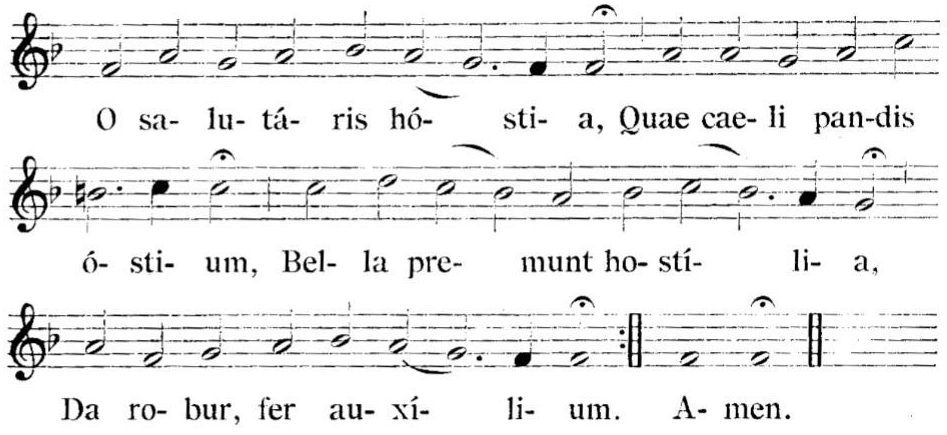
\includegraphics[width=\linewidth]{o-salutaris.jpg}
  \end{figure}

  \begin{center}
    \begin{footnotesize}
      \textit{
        Ô réconfortante
        Hostie, Qui nous
        ouvres les portes du
        ciel, les armées ennemies
        nous poursuivent,
        Donne-nous la force,
        porte-nous secours.
      }
    \end{footnotesize}
  \end{center}

  \begin{multicols}{2}
    \parindent=0pt
    \begin{flushright}
      O vere digna Hostia,\\
      Spes unica fidelium,\\
      In te confidit Francia,\\
      Da pacem, serva lilium.\\
    \end{flushright}
    \columnbreak
    \textit{
      Ô vraiment digne Hostie,\\
      Unique espoir des fidèles,\\
      en toi se confie la France,\\
      Donne-lui la paix, conserve le lys.\\
    }
  \end{multicols}
  \begin{multicols}{2}
    \begin{flushright}
      Uni trinoque Domino\\
      Sit sempiterna gloria :\\
      Qui vitam sine termino,\\
      Nobis donet in patria. Amen.\\
    \end{flushright}
    \columnbreak
    \textit{
      Au Seigneur unique en trois personnes,\\
      La gloire éternelle;\\
      qu'il nous donne en son Royaume\\
      La vie qui n'aura pas de fin. Amen\\
    }
  \end{multicols}

  \begin{center}
    \rule{2cm}{0.4pt}
  \end{center}

  \newpage

  \begin{center}
    \textcolor{red}{\large{Alma Redemptoris Mater}}\\
    \begin{footnotesize}
      \textit{
        Depuis les Vêpres du samedi avant le 1 Dimanche de l'Avent jusqu'aux Vêpres du 2 Février inclusivement.
      }
    \end{footnotesize}
  \end{center}

  \gresetinitiallines{1}
  \greillumination{\initfamily\fontsize{11mm}{11mm}\selectfont A}
  \gregorioscore{antiennes-mariales/an--alma_redemptoris--solesmes}
  \smallskip
  \begin{footnotesize}
    \textit{
      Mère féconde du Rédempteur, vous qui demeurez la Porte toujours ouverte du ciel et l'Étoile de la mer, venez au secours de ce peuple déchu qui voudrait se relever. Vous qui, au grand étonnement de la nature, avez donné le jour à votre divin Auteur, et qui êtes restée Vierge après comme auparavant, en recevant cet Ave de la bouche de Gabriel, ayez pitié des pécheurs.
    }
  \end{footnotesize}

  \begin{multicols}{2}
    \textcolor{red}{\Vbar.} Post partum, Virgo, invioláta\\ permansísti.\\
    \textcolor{red}{\Rbar.} Dei Génitrix, intercéde pro nobis.
  
    \columnbreak
    
    \textit{\textcolor{red}{\Vbar.} Après votre enfantement, ô Vierge, vous êtes
      demeurée sans tache.\\
      \textcolor{red}{\Rbar.} Mère de Dieu, intercédez pour nous.}
  \end{multicols}

  \begin{multicols}{2}
    \parindent=0pt
    Deus, qui salútis ætérnæ, beátæ Maríæ virginitáte fecúnda, humáno géneri præmia præstitísti :   \textcolor{red}{†} tríbue, quæsumus ; ut ipsam pro nobis intercédere sentiámus, per quam merúimus auctórem vitæ suscípere, \textcolor{red}{*} Dóminum nostrum Iesum Christum, Fílium tuum.
      \textcolor{red}{\Rbar.} Amen.

    \columnbreak
  
    \textit{ Dieu, qui par la virginité féconde de la
      bienheureuse Marie, avez procuré au genre
      humain les avantages du salut éternel ;
      accordez-nous, s’il vous plaît, de ressentir les
      effets de l’intercession de celle par qui nous
      avons eu la grâce de recevoir l’auteur de la vie,
      notre Seigneur Jésus-Christ, votre Fils. Amen.
      }
  \end{multicols}

  \begin{center}
    \rule{2cm}{0.4pt}
  \end{center}

  \newpage

  \begin{center}
    \textcolor{red}{\large{Ave Regina caelorum}}\\
    \begin{footnotesize}
      \textit{
      Depuis les Complies du 2 Février inclusivement, jusqu'aux Complies du Mercredi Saint inclusivement.
      }
    \end{footnotesize}
  \end{center}

  \gresetinitiallines{1}
  \greillumination{\initfamily\fontsize{11mm}{11mm}\selectfont A}
  \gregorioscore{antiennes-mariales/an--ave_regina_caelorum_(simple_tone)--solesmes}
  \medskip
  \begin{footnotesize}
    \textit{
      Salut, Reine des cieux ! Salut, Souveraine des Anges ! Salut, Tige, salut, Ô Porte par qui la lumière s'est levée sur le monde. Réjouissez-vous, Vierge glorieuse, qui l'emportez sur toutes en beauté ! Adieu, Ô toute belle, et priez le Christ pour nous.
    }
  \end{footnotesize}

  \begin{multicols}{2}
    \parindent=0pt
    \begin{flushright}
      \textcolor{red}{\Vbar.} Dignáre me laudáre te, Virgo sacráta.\\
      \textcolor{red}{\Rbar.} Da mihi virtútem contra hostes tuos.\\
    \end{flushright}
  
    \columnbreak
    
    \textit{\textcolor{red}{\Vbar.} Agréez que j’annonce vos louanges, Vierge
    sainte.\\
    \textcolor{red}{\Rbar.} Obtenez-moi la force contre vos ennemis.}\\
  \end{multicols}

  \begin{multicols}{2}
    \parindent=0pt
    Concede, miséricors Deus, fragilitáti nostræ præsídium :   \textcolor{red}{†} ut, qui sanctæ Dei Genitrícis memóriam ágimus ; \textcolor{red}{*} intercessiónis ejus
    auxílio, a nostris iniquitátibus resurgámus. Per Christum Dóminum nostrum.
    \textcolor{red}{\Rbar.} Amen.

    \columnbreak
  
    \textit{ Accordez, Dieu miséricordieux, à notre faiblesse les
      secours de votre grâce et comme nous célébrons la
      mémoire de la sainte Mère de Dieu, faites qu’étant
      aidés auprès de vous de son intercession, nous nous
      relevions de nos péchés. Par le Christ notre Seigneur.
      Amen.
    }
  \end{multicols}

  \begin{center}
    \rule{2cm}{0.4pt}
  \end{center}

  \begin{center}
    \textcolor{red}{\large{En l'honneur Du Saint Sacrement}}
  \end{center}

  \gresetinitiallines{1}
  \greillumination{\initfamily\fontsize{11mm}{11mm}\selectfont T}
  \gregorioscore{hymnes/hy--tantum_ergo--solesmes}

  \begin{center}
    \begin{footnotesize}
      \begin{enumerate}[label=\textcolor{red}{\emph{\arabic*}}]
        \item \textit{Devant un sacrement si grand, prosternons-nous, adorons ; et que les symboles anciens s'effacent devant le rite nouveau ; que la foi vienne suppléer à la faiblesse de nos sens.}
        \item \textit{Au Père et au Fils louanges et acclamations, gloire honneur et puissance ainsi que bénédictions. A Celui qui de tous deux procède offrons une égale louange.}
      \end{enumerate}
    \end{footnotesize}
  \end{center}

  \medskip

  \begin{multicols}{2}
    \parindent=0pt
    \textcolor{red}{\Vbar.} Panem de caelo praestitisti eis.\\
    \textcolor{red}{\Rbar.} Omne delectamentum in se habentem.\\
    
    \textit{\textcolor{red}{\Vbar.} Tu leur a donné le pain du ciel.\\
    \textcolor{red}{\Rbar.} Toute saveur se trouve en lui.}\\
    
  \end{multicols}

  \begin{center}
    \rule{2cm}{0.4pt}
  \end{center}

  \begin{center}
    \textcolor{red}{\large{Oraison}}
  \end{center}

  \begin{multicols}{2}
    \parindent=0pt
    Deus, qui nobis sub sacramento mirabili
    passionis tuæ memoriam reliquisti : \textcolor{red}{~†}
    tribue, quæsumus, ita nos Corporis et
    Sanguinis tui sacra mysteria venerari, \textcolor{red}{~*} ut
    redemptionis tuæ fructum in nobis
    jugiter sentiamus.\\
    Qui vivis et regnas
    cum Deo Patre in unitate Spiritus Sancti,
    Deus, per omnia sæcula sæculorum.
    Amen.
    \columnbreak

    \textit{
      Seigneur Jésus Christ, dans cet admirable
      sacrement tu nous a laissé le mémorial de
      ta passion ; donne-nous de vénérer d’un si
      grand amour le mystère de ton Corps et de
      ton Sang, que nous puissions recueillir
      sans cesse le fruit de ta rédemption. Toi
      qui règnes avec le Père et le Saint Esprit
      pour les siècles des siècles.
      Amen. 
    }
  \end{multicols}

  \begin{center}
    \rule{2cm}{0.4pt}
  \end{center}


  \begin{center}
    \textcolor{red}{\large{Louanges divines}}
  \end{center}


  \begin{normalsize}
    \parindent=0pt
    Dieu soit béni.\\
    Béni soit son Saint Nom.\\
    Béni soit Jésus-Christ, vrai Dieu et vrai homme.\\
    Béni soit le Nom de Jésus.\\
    Béni soit son Sacré Cœur.\\
    Béni soit son précieux Sang.\\
    Béni soit Jésus dans le très Saint Sacrement de l’autel.\\
    Béni soit l’Esprit Saint Consolateur.\\
    Bénie soit l’auguste Mère de Dieu, la très Sainte Vierge Marie.\\
    Bénie soit sa Sainte et Immaculée Conception.\\
    Bénie soit sa glorieuse Assomption.\\
    Béni soit le nom de Marie, Vierge et Mère.\\
    Béni soit Saint Joseph, son très chaste époux.\\
    Béni soit Dieu dans ses anges et dans ses saints.\\
    Seigneur, donnez-nous des prêtres.\\
    Seigneur, donnez-nous de saints prêtres.\\
    Seigneur, donnez-nous beaucoup de saints prêtres.\\
    Seigneur, donnez-nous beaucoup de saintes vocations religieuses.\\
  \end{normalsize}


  \newpage

  \begin{center}
    \textcolor{red}{\large{Déposition}}\\
    \textit{Psaume 116}
  \end{center}

  \gresetinitiallines{1}
  \greillumination{\initfamily\fontsize{11mm}{11mm}\selectfont L}
  \gregorioscore{../temps_pascal/psaumes/ps--laudate_dominum_omnes_gentes_(psalmus_116)--solesmes}
  \bigskip
  \begin{footnotesize}
    \textit{
      Louez le Seigneur, tous les
      peuples ;
      Fêtez-Le, tous les pays !
      Son Amour envers nous
      S'est montré le plus fort ;
      Eternelle est la Fidélité du
      Seigneur !
      Gloire au Père, au Fils
      Et au Saint-Esprit,
      Comme il était au
      commencement,
      Maintenant et toujours,
      Pour les siècles des siècles,
      amen.
    }
  \end{footnotesize}

\end{document}